
                \begin{figure}
                    \centering
                    \begin{tikzpicture}
                        \pgfplotsset{%
                            width=1\textwidth,
                            height=0.4\textheight
                        }
                        \begin{axis}[
                            xlabel={Runs since restart},
                            ylabel={Average dynamic energy (watt)},
                            ymin=0,ymax=70,
                        ]
                        
                            \addplot [mark=none, densely dashed, red]  coordinates {
                            (1, 41.67564618327381)(2, 39.68165239562263)(3, 39.65798152064811)(4, 40.78598578951857)(5, 40.50253578458274)
                            };
                            \addlegendentry{WRK - IPG}
                            
                            \addplot [mark=none, densely dashed, blue]  coordinates {
                            (1, 41.772671471799335)(2, 40.38545683070729)(3, 40.30687766861954)(4, 40.63625225322694)(5, 40.25174331481879)
                            };
                            \addlegendentry{WRK - LHM}
                            
                            \addplot [mark=none, densely dashed, cyan]  coordinates {
                            (1, 36.02602024964694)(2, 33.933571207200366)(3, 31.013160496170958)(4, 35.7314842561267)(5, 31.18544315034984)
                            };
                            \addlegendentry{WRK - CLAMP (win)}
                            
                            \addplot [mark=none, densely dashed, orange]  coordinates {
                            (1, 51.17521073003028)(2, 51.17796739108611)(3, 51.290363309915286)(4, 51.172453799525634)(5, 51.175882097019795)(6, 51.422685150207364)(9, 51.28231082237777)(10, 51.44563174116476)(11, 51.33525669951746)(12, 51.33491814357367)(14, 51.26243202899176)(15, 51.41706401911736)(17, 51.37397377830929)(18, 51.502815205547975)(19, 51.352383154264565)(20, 51.429570592492794)(21, 51.415379138248326)(23, 51.41110143010899)(24, 51.47843088489773)(25, 51.488381164078696)(26, 51.55041079478454)(27, 51.381958205481396)(28, 51.529191380000036)(29, 51.28481051597865)
                            };
                            \addlegendentry{WRK - RAPL}
                            
                            \addplot [mark=none, densely dashed, black]  coordinates {
                            (1, 53.05880185003335)(2, 48.49556066067936)(3, 43.58141531794655)(4, 44.151626660277884)(5, 44.410823145822704)(6, 43.818811817147264)(7, 43.80932986931859)(8, 43.91752532341533)(9, 44.78584035169021)(10, 44.175514919750825)(11, 44.089458242168135)(12, 44.33171588979198)(13, 44.515510261830215)(14, 44.79712064309405)(15, 44.77767627229544)(16, 44.70648576686044)(17, 33.29271431834104)(18, 44.349969988147535)(19, 44.344829488455176)(20, 44.61041779128158)(21, 44.918778034676805)(22, 44.54347760231637)(23, 44.31538241592479)(24, 44.89401380588265)(25, 44.264742315264016)(26, 43.504810440737245)(27, 43.966137181589914)(28, 43.79243471664576)(29, 43.9405242934896)
                            };
                            \addlegendentry{WRK - CLAMP (lin)}
                            
                        \end{axis}
                    \end{tikzpicture} 
                \caption{A graph illustrating the energy consumption of Cores for test case FannkuchRedux with regards to how long ago the DUT was restarted, experiment \#2, (without outliers)} \label{fig:FannkuchRedux_Cores_iteration_exp2}
                \end{figure}
                